\chapter{Results}
\label{ch:results}

%-------------------------------------------------------

This chapter reports the results of all experiments. All accuracies are on the synthetic test queries unless stated otherwise; real photos are covered in Section~\ref{sec:res-app}.

\section{Localisation and rectification}
\label{sec:res-rect}

The detector is the same for every retrieval method, so its accuracy on the test queries is a property of the query set. Figure~\ref{fig:pipeline-example} shows a typical successful case. On the \res{main-n-queries} single-card test queries per severity, the detected outline was correct (IoU $\geq 0.8$) for \res{rect-s1-ok}\%, \res{rect-s2-ok}\%, \res{rect-s3-ok}\%, \res{rect-s4-ok}\% and \res{rect-s5-ok}\% of the queries at severities 1 to 5. At severities 4 and 5 the detector returned a card outline at all for only \res{rect-s4-found}\% and \res{rect-s5-found}\% of the queries; in the remaining cases the pipeline fell back to the whole photo.

\begin{figure}[htbp]\centering
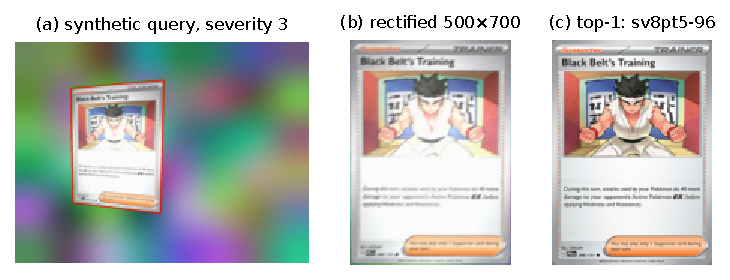
\includegraphics[width=\textwidth]{figures/pipeline_example.pdf}
\caption[Pipeline example]{Example run of the pipeline. (a) Synthetic query \texttt{s3\_0000}; green = true outline, red = outline found by the detector. (b) The card warped to the canonical view. (c) The reference scan ranked first by ORB + RANSAC (correct; 145 RANSAC inliers versus 67 for the second card).}\label{fig:pipeline-example}
\end{figure}


\section{Single-card identification (main comparison)}
\label{sec:res-main}

Table~\ref{tab:main} and Figure~\ref{fig:severity} show the strict and lenient top-1 accuracy of every method at every severity; Table~\ref{tab:main-detail} in Appendix~\ref{app:repro} adds top-5, MRR, 95\% confidence intervals and latencies.

\begin{table}[htbp]\centering\footnotesize
\caption[Top-1 accuracy per method and severity]{Top-1 identification accuracy on the synthetic single-card test queries (200 per severity), shown as strict / lenient. Strict = exact card id; lenient = any card with the same artwork (reprint). 95\% bootstrap intervals are in Table~\ref{tab:main-detail} and Figure~\ref{fig:severity}.}
\label{tab:main}
\begin{tabular}{@{}lccccc@{}}
\toprule
Method & S1 & S2 & S3 & S4 & S5\\
\midrule
Pixel thumbnail & 0.970 / 0.980 & 0.930 / 0.950 & 0.900 / 0.930 & 0.600 / 0.615 & 0.065 / 0.070\\
\midrule
ORB + RANSAC & 0.995 / 1.000 & 0.975 / 1.000 & 0.970 / 0.995 & 0.725 / 0.740 & 0.085 / 0.085\\
SIFT + RANSAC & 0.995 / 1.000 & 0.970 / 1.000 & 0.930 / 0.950 & 0.745 / 0.765 & 0.110 / 0.125\\
ResNet-50 & 0.970 / 0.995 & 0.780 / 0.800 & 0.375 / 0.380 & 0.120 / 0.120 & 0.025 / 0.025\\
CLIP ViT-B/32 & 0.970 / 1.000 & 0.955 / 0.995 & 0.845 / 0.875 & 0.250 / 0.255 & 0.020 / 0.020\\
Hybrid ResNet$\to$SIFT & 0.995 / 1.000 & 0.940 / 0.970 & 0.755 / 0.780 & 0.370 / 0.385 & 0.050 / 0.050\\
Hybrid CLIP$\to$SIFT & 0.995 / 1.000 & 0.965 / 0.995 & 0.935 / 0.955 & 0.530 / 0.535 & 0.020 / 0.020\\
ResNet-50 +rot & 0.970 / 0.995 & 0.745 / 0.760 & 0.340 / 0.345 & 0.130 / 0.130 & 0.030 / 0.030\\
CLIP +rot & 0.970 / 1.000 & 0.950 / 0.990 & 0.810 / 0.840 & 0.275 / 0.280 & 0.020 / 0.020\\
Hybrid ResNet$\to$SIFT +rot & 0.995 / 1.000 & 0.940 / 0.970 & 0.715 / 0.735 & 0.370 / 0.375 & 0.055 / 0.055\\
Hybrid CLIP$\to$SIFT +rot & 0.995 / 1.000 & 0.965 / 0.995 & 0.925 / 0.945 & 0.565 / 0.570 & 0.040 / 0.040\\
\bottomrule
\end{tabular}
\end{table}

\begin{figure}[htbp]\centering
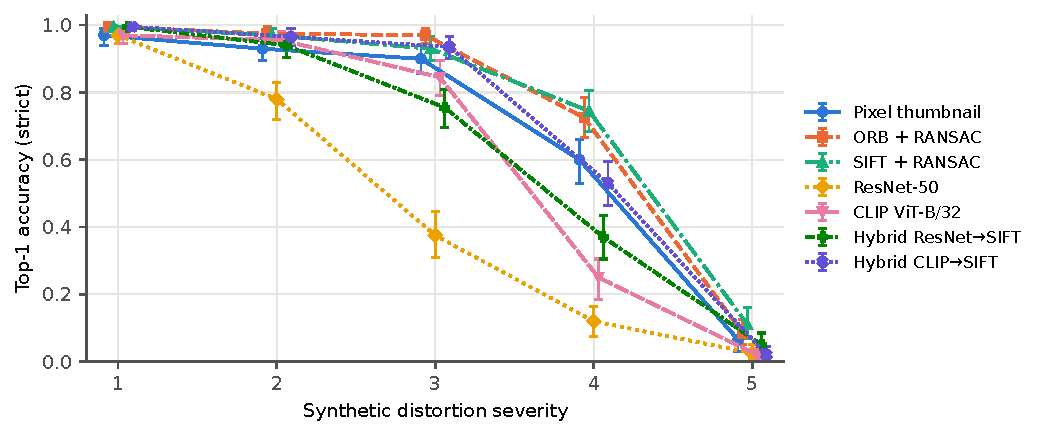
\includegraphics[width=\textwidth]{figures/accuracy_vs_severity.pdf}
\caption[Accuracy versus distortion severity]{Strict top-1 accuracy versus synthetic distortion severity for the seven base methods, with 95\% bootstrap intervals (200 queries per point; points slightly shifted horizontally for readability; the +rot variants are in Table~\ref{tab:main}).}\label{fig:severity}
\end{figure}


\paragraph{Mild distortion (severities 1--2).} All methods except ResNet-50 were close to perfect. At severity 1, ORB, SIFT and both hybrids reached a strict top-1 of \res{orb-s1-top1}, \res{sift-s1-top1}, \res{hybrid_resnet_k20-s1-top1} and \res{hybrid_clip_k20-s1-top1}, and ResNet-50 and CLIP \res{resnet-s1-top1} and \res{clip-s1-top1}. At severity 2 ResNet-50 already dropped to \res{resnet-s2-top1}, while CLIP kept \res{clip-s2-top1} and the CLIP hybrid \res{hybrid_clip_k20-s2-top1}. Under the lenient metric, ORB reached \res{orb-s1-top1_len} and \res{orb-s2-top1_len} and SIFT \res{sift-s1-top1_len} and \res{sift-s2-top1_len}, so every strict error of ORB and SIFT at these severities was a confusion with a reprint of the same artwork.

\paragraph{Moderate distortion (severity 3).} The methods separate clearly. ORB + RANSAC reached \res{orb-s3-top1} {\small[\res{orb-s3-top1_lo}, \res{orb-s3-top1_hi}]}, SIFT + RANSAC \res{sift-s3-top1} {\small[\res{sift-s3-top1_lo}, \res{sift-s3-top1_hi}]}, the CLIP hybrid \res{hybrid_clip_k20-s3-top1} {\small[\res{hybrid_clip_k20-s3-top1_lo}, \res{hybrid_clip_k20-s3-top1_hi}]}, CLIP alone \res{clip-s3-top1}, the ResNet hybrid \res{hybrid_resnet_k20-s3-top1} and ResNet-50 alone only \res{resnet-s3-top1}. Re-ranking the shortlist with SIFT therefore raised CLIP from \res{clip-s3-top1} to \res{hybrid_clip_k20-s3-top1} and ResNet-50 from \res{resnet-s3-top1} to \res{hybrid_resnet_k20-s3-top1}. The pixel-thumbnail baseline reached \res{pixel-s3-top1}, more than both global deep embeddings alone; this is discussed in Section~\ref{sec:disc-synthetic}.

\paragraph{Strong distortion (severities 4--5).} At severity 4, the two exhaustive keypoint methods remained best, SIFT with \res{sift-s4-top1} {\small[\res{sift-s4-top1_lo}, \res{sift-s4-top1_hi}]} and ORB with \res{orb-s4-top1} {\small[\res{orb-s4-top1_lo}, \res{orb-s4-top1_hi}]} (overlapping intervals), followed by the pixel baseline (\res{pixel-s4-top1}), the CLIP hybrid with rotation (\res{hybrid_clip+rot_k20-s4-top1}) and without (\res{hybrid_clip_k20-s4-top1}), the ResNet hybrid (\res{hybrid_resnet_k20-s4-top1}), CLIP (\res{clip-s4-top1}) and ResNet-50 (\res{resnet-s4-top1}). At severity 5 every method failed (strict top-1 between \res{clip-s5-top1} for CLIP and \res{sift-s5-top1} for SIFT), because the card outline was found correctly in only \res{rect-s5-ok}\% of these photos (Section~\ref{sec:failures}).

\paragraph{Trying both orientations (+rot).} Embedding the query also rotated by $180^\circ$ removed every ``upside down'' failure (Table~\ref{tab:failures}), but it did not improve the accuracy: at severity 3 it was slightly lower for every embedding method (for example CLIP \res{clip+rot-s3-top1} versus \res{clip-s3-top1}, CLIP hybrid \res{hybrid_clip+rot_k20-s3-top1} versus \res{hybrid_clip_k20-s3-top1}), and at severity 4 slightly higher for CLIP and its hybrid (\res{clip+rot-s4-top1} versus \res{clip-s4-top1}, \res{hybrid_clip+rot_k20-s4-top1} versus \res{hybrid_clip_k20-s4-top1}); in every case the 95\% intervals of the two variants overlap. A plausible explanation is that comparing each reference with two versions of the query also doubles the chances of a wrong card scoring high. In the failure analysis, pooled over all severities, the number of failures with and without +rot was \res{fail-resnet+rot-total} versus \res{fail-resnet-total} for ResNet-50, \res{fail-clip+rot-total} versus \res{fail-clip-total} for CLIP, \res{fail-hybrid_resnet+rot_k20-total} versus \res{fail-hybrid_resnet_k20-total} for the ResNet hybrid and \res{fail-hybrid_clip+rot_k20-total} versus \res{fail-hybrid_clip_k20-total} for the CLIP hybrid: the upside-down failures disappear, but other failures take most of their place.

\paragraph{ORB versus SIFT.} The two keypoint methods were statistically tied at every severity: ORB was slightly ahead at severity 3 (\res{orb-s3-top1} versus \res{sift-s3-top1}) and SIFT slightly ahead at severities 4 and 5 (\res{sift-s4-top1} versus \res{orb-s4-top1}, \res{sift-s5-top1} versus \res{orb-s5-top1}), with overlapping 95\% intervals in every case. Both match the query against all \res{db-cards} reference cards, which took several seconds per photo on the test laptop (median \res{orb-s3-ms}~ms for ORB and \res{sift-s3-ms}~ms for SIFT at severity 3).

\section{Shortlist size of the hybrid}
\label{sec:res-ksweep}

Figure~\ref{fig:ksweep} shows how the shortlist size $k$ trades accuracy for time at severity 3. For the CLIP hybrid the shortlist matters little: strict top-1 grew from \res{ks-clip-k5-top1} with $k=5$ (median \res{ks-clip-k5-ms}~ms per photo) to \res{ks-clip-k20-top1} with $k=20$ (\res{ks-clip-k20-ms}~ms) and \res{ks-clip-k50-top1} with $k=50$ (\res{ks-clip-k50-ms}~ms). Already with $k=20$ the hybrid matched exhaustive SIFT (\res{sift-s3-top1}, median \res{sift-s3-ms}~ms per photo), which uses exactly the same SIFT verification but against all \res{db-cards} cards instead of 20; with $k=50$ its 95\% interval {\small[\res{ks-clip-k50-top1_lo}, \res{ks-clip-k50-top1_hi}]} also overlaps that of exhaustive ORB (\res{orb-s3-top1} {\small[\res{orb-s3-top1_lo}, \res{orb-s3-top1_hi}]}, median \res{orb-s3-ms}~ms), in a fraction of the time. For the ResNet hybrid the shortlist is decisive: \res{ks-resnet-k5-top1} with $k=5$, \res{ks-resnet-k20-top1} with $k=20$ and \res{ks-resnet-k50-top1} with $k=50$, because ResNet-50 often does not rank the correct card among its first few candidates, and SIFT can only choose among the cards it is given.

\begin{figure}[htbp]\centering
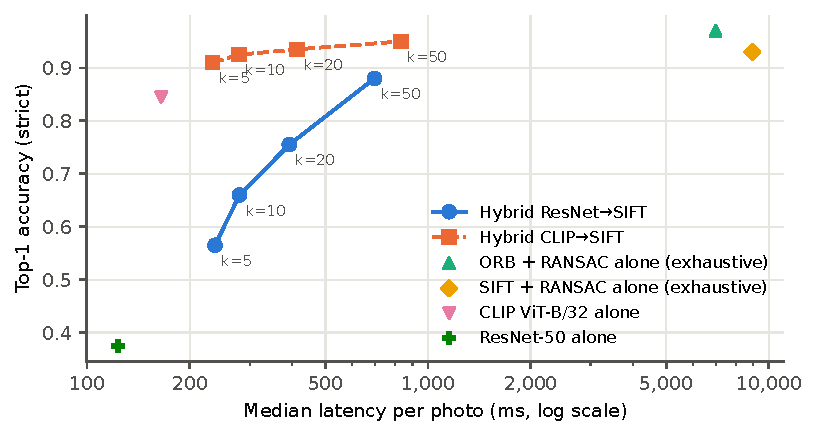
\includegraphics[width=\textwidth]{figures/ksweep.pdf}
\caption{Hybrid shortlist size $k$ (5, 10, 20, 50) at severity 3: accuracy versus median latency, compared with each component alone.}\label{fig:ksweep}
\end{figure}


\section{Effect of rectification}
\label{sec:res-norect}

Table~\ref{tab:norectify} compares each method at severity 3 with and without the rectification step. Without it, the global methods collapsed: the CLIP hybrid fell from \res{hybrid_clip_k20-s3-top1} to \res{norect-hybrid_clip_k20-top1}, CLIP from \res{clip-s3-top1} to \res{norect-clip-top1}, ResNet-50 from \res{resnet-s3-top1} to \res{norect-resnet-top1} and the pixel baseline from \res{pixel-s3-top1} to \res{norect-pixel-top1}. In these photos the card covers only part of the image and is rotated and seen in perspective; resizing the whole photo leaves most of the image as background, which dominates a global descriptor. The keypoint methods degraded less: SIFT kept \res{norect-sift-top1} (from \res{sift-s3-top1}) and ORB \res{norect-orb-top1} (from \res{orb-s3-top1}). Their features are local and invariant to rotation and scale, and the RANSAC homography can itself absorb the perspective, so they do not need the card to fill the image; they still lose most of their accuracy, because the small, unrectified card provides far fewer keypoints. Rectification is therefore a necessary step for every method, and essential for the global ones.

\begin{table}[htbp]\centering\small
\caption[Rectification ablation]{Ablation at severity 3: strict top-1 with rectification versus the whole photo resized to the canonical size.}\label{tab:norectify}
\begin{tabular}{@{}lcc@{}}
\toprule
Method & Rectified & Whole photo\\
\midrule
Pixel thumbnail & 0.900 & 0.005\\
ORB + RANSAC & 0.970 & 0.165\\
SIFT + RANSAC & 0.930 & 0.425\\
ResNet-50 & 0.375 & 0.005\\
CLIP ViT-B/32 & 0.845 & 0.020\\
Hybrid ResNet$\to$SIFT & 0.755 & 0.090\\
Hybrid CLIP$\to$SIFT & 0.935 & 0.080\\
ResNet-50 +rot & 0.340 & 0.005\\
CLIP +rot & 0.810 & 0.025\\
Hybrid ResNet$\to$SIFT +rot & 0.715 & 0.100\\
Hybrid CLIP$\to$SIFT +rot & 0.925 & 0.075\\
\bottomrule
\end{tabular}
\end{table}


\section{Multi-card scenes}
\label{sec:res-scenes}

Table~\ref{tab:scenes} reports the scenes with 2--6 cards at severity 2. Detection is the same for every method. With no overlap the detector found \res{sc-o0-recall} of the cards with a precision of \res{sc-o0-precision}; with up to 15\% and 30\% overlap, recall fell to \res{sc-o15-recall} and \res{sc-o30-recall}. The best end-to-end result (card detected \emph{and} correctly identified) was obtained by the CLIP hybrid: \res{sc-hybrid_clip_k20-o0-e2e_top1} without overlap, \res{sc-hybrid_clip_k20-o15-e2e_top1} and \res{sc-hybrid_clip_k20-o30-e2e_top1} with overlap. Among the cards that were detected, the CLIP hybrid identified \res{sc-hybrid_clip_k20-o0-id_acc_given_detected} correctly without overlap, so the loss comes mostly from detection: overlapping cards merge into one contour, as expected from the design of the detector (Section~\ref{sec:localisation}).

\begin{table}[htbp]\centering\small
\caption[Multi-card scenes]{Multi-card synthetic scenes (severity 2): detection precision / recall / F1 (IoU $\geq$ 0.5) and end-to-end top-1 (detected and correctly identified / all cards).}\label{tab:scenes}
\begin{tabular}{@{}lccccc@{}}
\toprule
Method & Overlap & P & R & F1 & End-to-end top-1\\
\midrule
ResNet-50 & 0\% & 0.911 & 0.706 & 0.795 & 0.349 {\scriptsize[0.30, 0.40]}\\
ResNet-50 & 15\% & 0.759 & 0.330 & 0.460 & 0.168 {\scriptsize[0.13, 0.20]}\\
ResNet-50 & 30\% & 0.721 & 0.291 & 0.415 & 0.154 {\scriptsize[0.12, 0.19]}\\
CLIP ViT-B/32 & 0\% & 0.911 & 0.706 & 0.795 & 0.571 {\scriptsize[0.52, 0.62]}\\
CLIP ViT-B/32 & 15\% & 0.759 & 0.330 & 0.460 & 0.267 {\scriptsize[0.22, 0.31]}\\
CLIP ViT-B/32 & 30\% & 0.721 & 0.291 & 0.415 & 0.220 {\scriptsize[0.18, 0.26]}\\
Hybrid ResNet$\to$SIFT & 0\% & 0.911 & 0.706 & 0.795 & 0.574 {\scriptsize[0.53, 0.63]}\\
Hybrid ResNet$\to$SIFT & 15\% & 0.759 & 0.330 & 0.460 & 0.275 {\scriptsize[0.23, 0.32]}\\
Hybrid ResNet$\to$SIFT & 30\% & 0.721 & 0.291 & 0.415 & 0.240 {\scriptsize[0.20, 0.28]}\\
Hybrid CLIP$\to$SIFT & 0\% & 0.911 & 0.706 & 0.795 & 0.643 {\scriptsize[0.59, 0.69]}\\
Hybrid CLIP$\to$SIFT & 15\% & 0.759 & 0.330 & 0.460 & 0.285 {\scriptsize[0.24, 0.33]}\\
Hybrid CLIP$\to$SIFT & 30\% & 0.721 & 0.291 & 0.415 & 0.247 {\scriptsize[0.21, 0.29]}\\
\bottomrule
\end{tabular}
\end{table}


\section{Identification across printed languages}
\label{sec:res-language-id}

In this experiment SIFT, CLIP and the CLIP hybrid were run on the same English, Spanish and Japanese queries (Table~\ref{tab:language-id}). All queries are at severity 2, so the in-plane rotation is at most $15^\circ$ and the upside-down problem does not occur.

\begin{table}[htbp]\centering\footnotesize
\caption[Identification per printed language]{Lenient top-1 identification per printed language (test split, severity 2) with 95\% bootstrap intervals, at two photo resolutions: card about 530~px tall (``low'') and about 1050~px tall (``phone'', like a 12~MP photo). @art = only the artwork window is compared; +rot = the query is also tried rotated 180\textdegree. Queries: en 60, es 60, ja 43.}\label{tab:language-id}
\begin{tabular}{@{}lllll@{}}
\toprule
Method & Res. & English & Spanish & Japanese\\
\midrule
SIFT + RANSAC & low & 1.000 {\scriptsize[1.00, 1.00]} & 1.000 {\scriptsize[1.00, 1.00]} & 1.000 {\scriptsize[1.00, 1.00]}\\
 & phone & 1.000 {\scriptsize[1.00, 1.00]} & 1.000 {\scriptsize[1.00, 1.00]} & 0.977 {\scriptsize[0.93, 1.00]}\\
\addlinespace[2pt]
SIFT + RANSAC @art & low & 1.000 {\scriptsize[1.00, 1.00]} & 1.000 {\scriptsize[1.00, 1.00]} & 1.000 {\scriptsize[1.00, 1.00]}\\
 & phone & 1.000 {\scriptsize[1.00, 1.00]} & 1.000 {\scriptsize[1.00, 1.00]} & 1.000 {\scriptsize[1.00, 1.00]}\\
\addlinespace[2pt]
CLIP ViT-B/32 & low & 0.983 {\scriptsize[0.95, 1.00]} & 0.883 {\scriptsize[0.80, 0.95]} & 0.628 {\scriptsize[0.49, 0.77]}\\
 & phone & 1.000 {\scriptsize[1.00, 1.00]} & 0.967 {\scriptsize[0.92, 1.00]} & 0.767 {\scriptsize[0.65, 0.88]}\\
\addlinespace[2pt]
CLIP @art & low & 0.933 {\scriptsize[0.87, 0.98]} & 1.000 {\scriptsize[1.00, 1.00]} & 0.767 {\scriptsize[0.63, 0.88]}\\
 & phone & 0.967 {\scriptsize[0.92, 1.00]} & 1.000 {\scriptsize[1.00, 1.00]} & 0.860 {\scriptsize[0.74, 0.95]}\\
\addlinespace[2pt]
Hybrid CLIP$\to$SIFT +rot & low & 0.983 {\scriptsize[0.95, 1.00]} & 0.950 {\scriptsize[0.88, 1.00]} & 0.930 {\scriptsize[0.84, 1.00]}\\
 & phone & 1.000 {\scriptsize[1.00, 1.00]} & 0.950 {\scriptsize[0.88, 1.00]} & 1.000 {\scriptsize[1.00, 1.00]}\\
\addlinespace[2pt]
Hybrid CLIP$\to$SIFT @art +rot & low & 1.000 {\scriptsize[1.00, 1.00]} & 1.000 {\scriptsize[1.00, 1.00]} & 0.884 {\scriptsize[0.77, 0.98]}\\
 & phone & 1.000 {\scriptsize[1.00, 1.00]} & 1.000 {\scriptsize[1.00, 1.00]} & 0.977 {\scriptsize[0.93, 1.00]}\\
\addlinespace[2pt]
\bottomrule
\end{tabular}
\end{table}


\begin{itemize}
  \item \textbf{SIFT + RANSAC} was almost unaffected by the printed language: its lenient top-1 was between \res{lang-sift-ja-hr-len} and \res{lang-sift-en-low-len} in every language and at both resolutions, with or without the artwork crop.
  \item \textbf{CLIP} depended on the language: at low resolution its lenient top-1 was \res{lang-clip-en-low-len} for English, \res{lang-clip-es-low-len} for Spanish and \res{lang-clip-ja-low-len} for Japanese cards (phone resolution: \res{lang-clip-en-hr-len}, \res{lang-clip-es-hr-len}, \res{lang-clip-ja-hr-len}). Restricting CLIP to the artwork window gave \res{lang-clip@art-ja-low-len} (low) and \res{lang-clip@art-ja-hr-len} (phone) on Japanese cards, but with only \res{lang-ja-n} Japanese queries the confidence intervals of CLIP and CLIP@art overlap.
  \item \textbf{The CLIP hybrid} with SIFT re-ranking reached \res{lang-hybrid_clip+rot_k20-ja-low-len} (low) and \res{lang-hybrid_clip+rot_k20-ja-hr-len} (phone) on Japanese cards; the artwork-only hybrid reached \res{lang-hybrid_clip@art+rot_k20-ja-low-len} and \res{lang-hybrid_clip@art+rot_k20-ja-hr-len}.
  \item \textbf{Cost.} The median time per photo at phone resolution, pooled over the three languages, was \res{lang-clip-ms}~ms for CLIP, \res{lang-hybrid_clip+rot_k20-ms}~ms for the CLIP hybrid, \res{lang-sift@art-ms}~ms for SIFT@art and \res{lang-sift-ms}~ms for exhaustive SIFT (indicative only, see the latency note in Chapter~\ref{ch:data}). The index of SIFT needs \res{index-sift-MB}~MB, the index of CLIP \res{index-clip-MB}~MB.
\end{itemize}

\section{Printed-language classification}
\label{sec:res-language-clf}

Table~\ref{tab:language-clf} and Figure~\ref{fig:language-confusion} report the OCR-based language classifier. The first version of the rules, fixed before looking at any data and evaluated once on the test split at low resolution, reached an accuracy of \res{langclf-v1-test-acc}: \res{langclf-v1-test-unknown} cards were ``unknown'' and \res{langclf-v1-test-wrong} were assigned to another language. The second version (kana-only script test, language-code box, phone resolution, OCR at $750\times1050$) was tuned on the development split (\res{langclf-v2-dev-acc}) and then evaluated once on the test split: \res{langclf-v2-test-acc} {\small[\res{langclf-v2-test-lo}, \res{langclf-v2-test-hi}]}, with \res{langclf-v2-test-unknown} ``unknown'' answers and \res{langclf-v2-test-wrong} confusions between languages.

\begin{table}[htbp]\centering\small
\caption[Printed-language classification]{Printed-language classification (English / Spanish / Japanese) with OCR + rules. Version 1 rules were fixed before seeing any data; version 2 was tuned on the dev split only. ``Unknown'' = no usable text; ``wrong'' = another language predicted.}\label{tab:language-clf}
\begin{tabular}{@{}lllrcrr@{}}
\toprule
Rules & Split & Res. & $n$ & Accuracy [95\% CI] & Unknown & Wrong\\
\midrule
v1 & test & low & 180 & 0.539 {\scriptsize[0.46, 0.61]} & 66 & 17\\
v2 & dev & phone & 180 & 0.928 {\scriptsize[0.89, 0.96]} & 13 & 0\\
v2 & test & phone & 180 & 0.911 {\scriptsize[0.87, 0.95]} & 14 & 2\\
\bottomrule
\end{tabular}
\end{table}


\begin{figure}[htbp]\centering
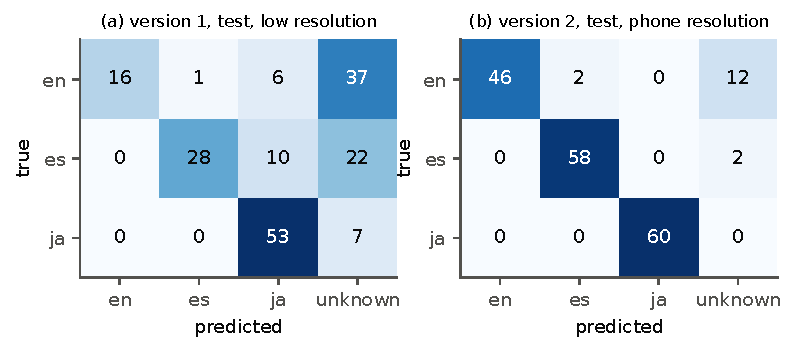
\includegraphics[width=\textwidth]{figures/language_confusion.pdf}
\caption[Language confusion matrices]{Confusion matrices of the printed-language classifier on the test split (rows: true language; columns: predicted language or ``unknown'').}
\label{fig:language-confusion}
\end{figure}

\section{Condition estimate}
\label{sec:res-condition}

Table~\ref{tab:condition} summarises the validation on synthetically damaged cards and Figure~\ref{fig:condition-example} shows an example. Centering was measured with a median error of \res{cond-centering-lr-med} (left/right) and \res{cond-centering-tb-med} (top/bottom) percentage points. Corner cuts, corner whitening and edge whitening correlated clearly with their sub-scores ($\rho$ = \res{cond-rho-corner-cut}, \res{cond-rho-corner-white}, \res{cond-rho-edge-white}), edge fraying less so ($\rho$ = \res{cond-rho-edge-fray}). Surface defects were found with a recall of \res{cond-surf-recall} and a precision of \res{cond-surf-precision}.

\begin{table}[htbp]\centering\small
\caption[Condition estimate validation]{Validation of the visual condition estimate on 80 test cards with synthetic damage of known strength (front side only). $\rho$ = Spearman rank correlation between true damage strength and the estimate.}\label{tab:condition}
\begin{tabular}{@{}lr@{}}
\toprule
Measure & Result\\
\midrule
Cards rectified / reference aligned & 80 / 76\\
Centering error L/R, median / 90th pct.\ (percentage points) & 0.58 / 2.33\\
Centering error T/B, median / 90th pct.\ (percentage points) & 0.70 / 2.33\\
$\rho$ corner cut vs.\ fill sub-score (expect $<0$) & -0.74\\
$\rho$ corner whitening vs.\ whitening sub-score & +0.62\\
$\rho$ edge whitening vs.\ whitening sub-score & +0.78\\
$\rho$ edge fray vs.\ fray sub-score & +0.41\\
Surface defects: recall / precision & 68/111 = 0.61 / 72/105 = 0.69\\
Surface defects with correct type & 59/111\\
$\rho$ part score vs.\ true damage: corners / edges / surface / centering & -0.53 / -0.32 / -0.86 / -0.90\\
$\rho$ overall score vs.\ total damage & -0.46\\
\bottomrule
\end{tabular}
\end{table}


\begin{figure}[htbp]\centering
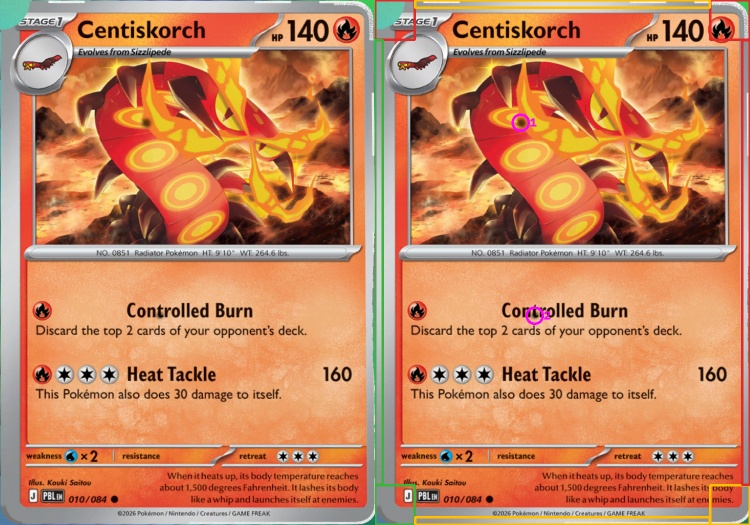
\includegraphics[width=0.85\textwidth]{figures/condition_example.jpg}
\caption[Condition estimate example]{Condition estimate on a synthetically damaged test card. Left: the rectified photo. Right: the same photo with the analysed corner and edge zones and the detected surface defects marked.}
\label{fig:condition-example}
\end{figure}

The back side could not be validated in the same way, because no official scans of card backs exist; the application's results on real photos follow in Section~\ref{sec:res-app}.

\section{The application on real photos}
\label{sec:res-app}

At the end of the project the CardDex collection contains \res{app-n-items} cards that were identified from real photos and saved by the author: \res{app-n-en} English cards and \res{app-n-ja} Japanese cards from \emph{Battle Partners} (Table~\ref{tab:app-collection}; snapshot of \res{app-snapshot-date}). Their stored prices add up to USD~\res{app-total-usd} for the English cards and EUR~\res{app-total-eur} for the Japanese cards (prices change daily; the two currencies are kept apart). Each saved card keeps the photo it was identified from (Figure~\ref{fig:app-photos}). Most of them are phone photos of cards inside protective sleeves or rigid holders, lying on a keyboard, which is a realistic and difficult setting for the detector. The Mega Chandelure is a Japanese print of a \emph{Pitch Black} card; Japanese scans of that set were not available, so it can only match its English version, and its image looks like a clean scan rather than a phone photo.

\begin{table}[htbp]\centering\footnotesize
\caption[Cards saved in the application]{Cards saved in the CardDex collection (snapshot of 2026-11-08). Price when saved: English cards = mean TCGplayer market price of the card's variants in USD; Japanese cards = Cardmarket average in EUR (both via TCGdex). Score of the saved card with the method used at save time: RANSAC inliers for SIFT, ORB and the hybrids, cosine similarity in \% for ResNet and CLIP. Condition: overall visual estimate (0--1000; mean of the two sides) and the front / back side scores as stored by the app (-- = not assessed). Lang.: printed language stored with the item.}\label{tab:app-collection}
\begin{tabular}{@{}P{1.45in}P{1.05in}cP{0.6in}rrP{1.15in}@{}}
\toprule
Card (id) & Rarity & Lang. & Method & Price & Score & Condition (overall; front / back)\\
\midrule
Mega Chandelure ex (\texttt{me5-115}) & Special Illustration Rare & en & sift & USD 32.39 & 59 & 320; 167 / 473\\
Morpeko ex (\texttt{me5-102}) & Ultra Rare & en & hybrid CLIP +rot & USD 3.52 & 285 & 258; 269 / 246\\
Goldeen (\texttt{me5-87}) & Illustration Rare & en & sift & USD 3.51 & 202 & 150; 198 / 103\\
Toucannon (\texttt{me5-94}) & Illustration Rare & en & resnet & USD 1.55 & 82.9 & 132; 162 / 103\\
Thievul (\texttt{me5-92}) & Illustration Rare & en & resnet & USD 1.31 & 76.9 & 136; 170 / 103\\
Maractus (JP) (\texttt{ja-SV9-101}) & -- & ja & sift & EUR 1.33 & 251 & 261; 220 / 302\\
Swinub (JP) (\texttt{ja-SV9-106}) & -- & ja & sift & EUR 1.60 & 290 & 189; 197 / 181\\
\bottomrule
\end{tabular}
\end{table}

\begin{figure}[htbp]\centering
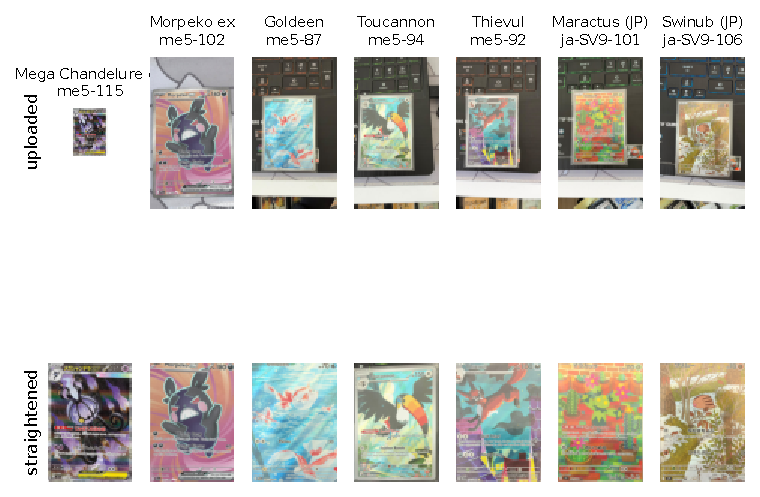
\includegraphics[width=\textwidth]{figures/app_photos.pdf}
\caption[Photos saved in the application]{The photos stored with the saved cards (top) and the card image that the application straightened from each one and passed to the retrieval method (bottom).}\label{fig:app-photos}
\end{figure}


\paragraph{Re-identification.} To turn the saved photos into a small real-photo test, every photo was identified again with each method, through the same code path as the application and against all \res{app-n-ref} reference cards of the application (\texttt{report/app\_evidence.py}). The ground truth is the card that the user saved, which the application lets the user correct before saving. Table~\ref{tab:app-reid} shows the result.
\begin{itemize}
  \item SIFT, ORB, CLIP and the CLIP hybrid ranked the exact saved card first for all \res{app-reid-n} photos, including both Japanese cards, which were matched to their Japanese scan and not to their English twin.
  \item ResNet-50 was correct for \res{app-resnet-hits} of \res{app-reid-n} photos (\res{app-resnet-hits-len} under the lenient metric): it ranked the Morpeko ex at position \res{app-resnet-me5-102-rank}, and it returned the English twin (\texttt{\res{app-resnet-ja-SV9-101-pred}}) for the Japanese Maractus.
  \item The artwork-only hybrid found the right artwork every time (\res{app-hybrid_clip@art+rot_k20-hits-len} of \res{app-reid-n} lenient) but returned the English twin for both Japanese cards (\res{app-hybrid_clip@art+rot_k20-hits} of \res{app-reid-n} strict). This is exactly what the method is designed to do: it ignores the text, and the text is the only difference between the two prints.
  \item SIFT separated the correct card clearly in every case, for example \res{app-me5-87-sift-top1} RANSAC inliers for Goldeen against \res{app-me5-87-sift-second} for the second card, and \res{app-ja-SV9-101-sift-top1} against \res{app-ja-SV9-101-sift-second} for the Japanese Maractus.
  \item Median time per photo: \res{app-sift-ms}~ms for SIFT, \res{app-orb-ms}~ms for ORB, \res{app-clip-ms}~ms for CLIP and \res{app-hybrid_clip+rot_k20-ms}~ms for the CLIP hybrid. These timings were taken while the main experiments were running on the same laptop and are only indicative.
\end{itemize}
With \res{app-reid-n} photos these numbers illustrate the behaviour on real photos but are not a statistical result.

\begin{table}[htbp]\centering\footnotesize
\caption[Re-identification of the saved photos]{Re-identification of the photos saved in the application with every method (same path as the app: rectification, then ranking of all 917 reference cards of the app, English and Japanese). Each cell is the rank of the saved card (1 = correct top-1); $\dagger$ = wrong exact card but same artwork (lenient top-1, e.g.\ the English twin of a Japanese card); bold = wrong even under the lenient metric. Ground truth = the card the user saved. Top-1 = strict / lenient. Latency: median over the photos (measured while other experiments were running, indicative only).}\label{tab:app-reid}
\begin{tabular}{@{}lcccccccrr@{}}
\toprule
Method & \rotatebox{70}{Mega Chandelure ex} & \rotatebox{70}{Morpeko ex} & \rotatebox{70}{Goldeen} & \rotatebox{70}{Toucannon} & \rotatebox{70}{Thievul} & \rotatebox{70}{Maractus (JP)} & \rotatebox{70}{Swinub (JP)} & Top-1 & ms\\
\midrule
Pixel thumbnail & 1 & 1 & \textbf{2} & 1 & \textbf{22} & \textbf{32} & \textbf{7} & 3/3 & 142\\
SIFT + RANSAC & 1 & 1 & 1 & 1 & 1 & 1 & 1 & 7/7 & 22,329\\
ORB + RANSAC & 1 & 1 & 1 & 1 & 1 & 1 & 1 & 7/7 & 7,064\\
ResNet-50 & 1 & \textbf{191} & 1 & 1 & 1 & 2$^\dagger$ & 1 & 5/6 & 275\\
CLIP ViT-B/32 & 1 & 1 & 1 & 1 & 1 & 1 & 1 & 7/7 & 270\\
Hybrid CLIP$\to$SIFT +rot & 1 & 1 & 1 & 1 & 1 & 1 & 1 & 7/7 & 1,015\\
Hybrid CLIP$\to$SIFT @art +rot & 1 & 1 & 1 & 1 & 1 & 2$^\dagger$ & 2$^\dagger$ & 5/7 & 735\\
\bottomrule
\end{tabular}
\end{table}


\paragraph{Detection on real photos.} The detector returned an outline for every saved photo, but on sleeved cards the outline is not always the card edge (Figure~\ref{fig:app-photos}): for several cards the straightened image is cropped slightly inside the card border, and for the Toucannon it includes part of the sleeve. A likely reason is that the detector keeps the strongest card-shaped rectangle, and a sleeve or rigid holder adds further rectangles just inside and outside the card edge. Identification was not affected, because the artwork and most of the card remained inside the warped image.

\paragraph{Condition estimates on real photos.} The stored condition estimates were low for every card (overall between \res{app-cond-min} and \res{app-cond-max} out of 1000), and several fronts were reported with many surface ``defects'' (for example \res{app-me5-115-front-ndefects} for the Mega Chandelure, compared with the English scan, and \res{app-ja-SV9-101-front-ndefects} for the Japanese Maractus, compared with its own Japanese scan). The Goldeen, Toucannon and Thievul have identical back scores (\res{app-me5-87-back-overall}), which suggests that the same back photo was used for the three cards. The true condition of these cards was not recorded, so the estimates cannot be scored; they are discussed in Section~\ref{sec:disc-app}.

\section{Real photos (systematic evaluation)}
\label{sec:res-real}

The planned systematic real-photo set (70--100 labelled phone photos per set under controlled variations, Section~\ref{sec:realphotos}) was not collected within the project. The real-photo evidence of this report is therefore limited to the \res{app-reid-n} photos saved in the application (Section~\ref{sec:res-app}); this is listed as a limitation in Chapter~\ref{ch:conclusions}.
